\section{Additional Data}
To illustrate the very similar statistics obtained by the different mapping schemes described and discussed in section \ref{sec:NumConve}, in Figure \ref{appFig:SchemHist} further properties are shown, each normalised for better comparatibility.
In the figures, the radius-edge ratio denotes the ratio of the radius of circumsphere divided by the sortest edge length.
\begin{figure}
\begin{subfigure}{0.5\textwidth}
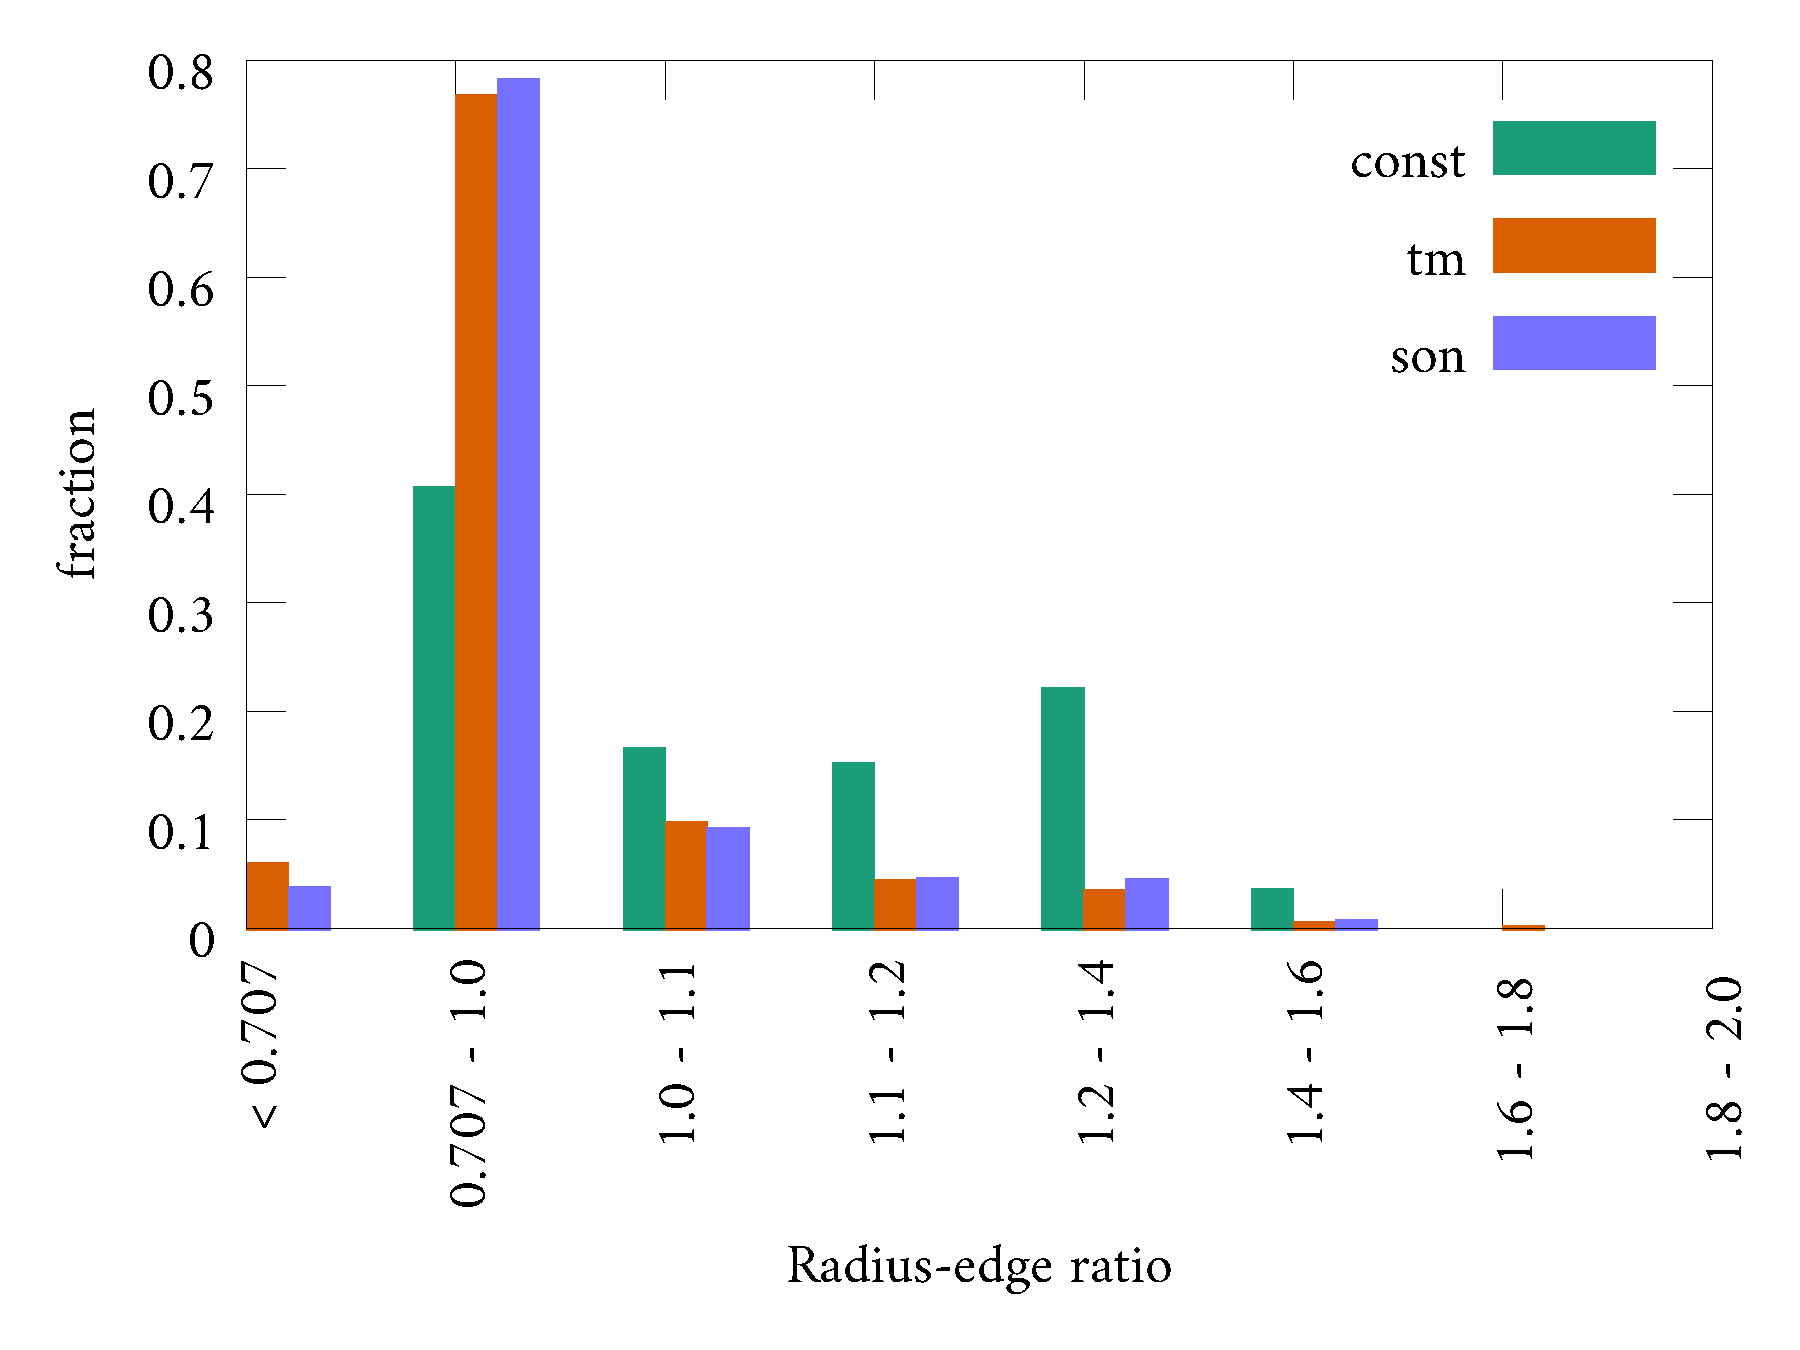
\includegraphics[width=\textwidth]{Figures/App/Rad_histAp1.pdf}
\end{subfigure}
\begin{subfigure}{0.5\textwidth}
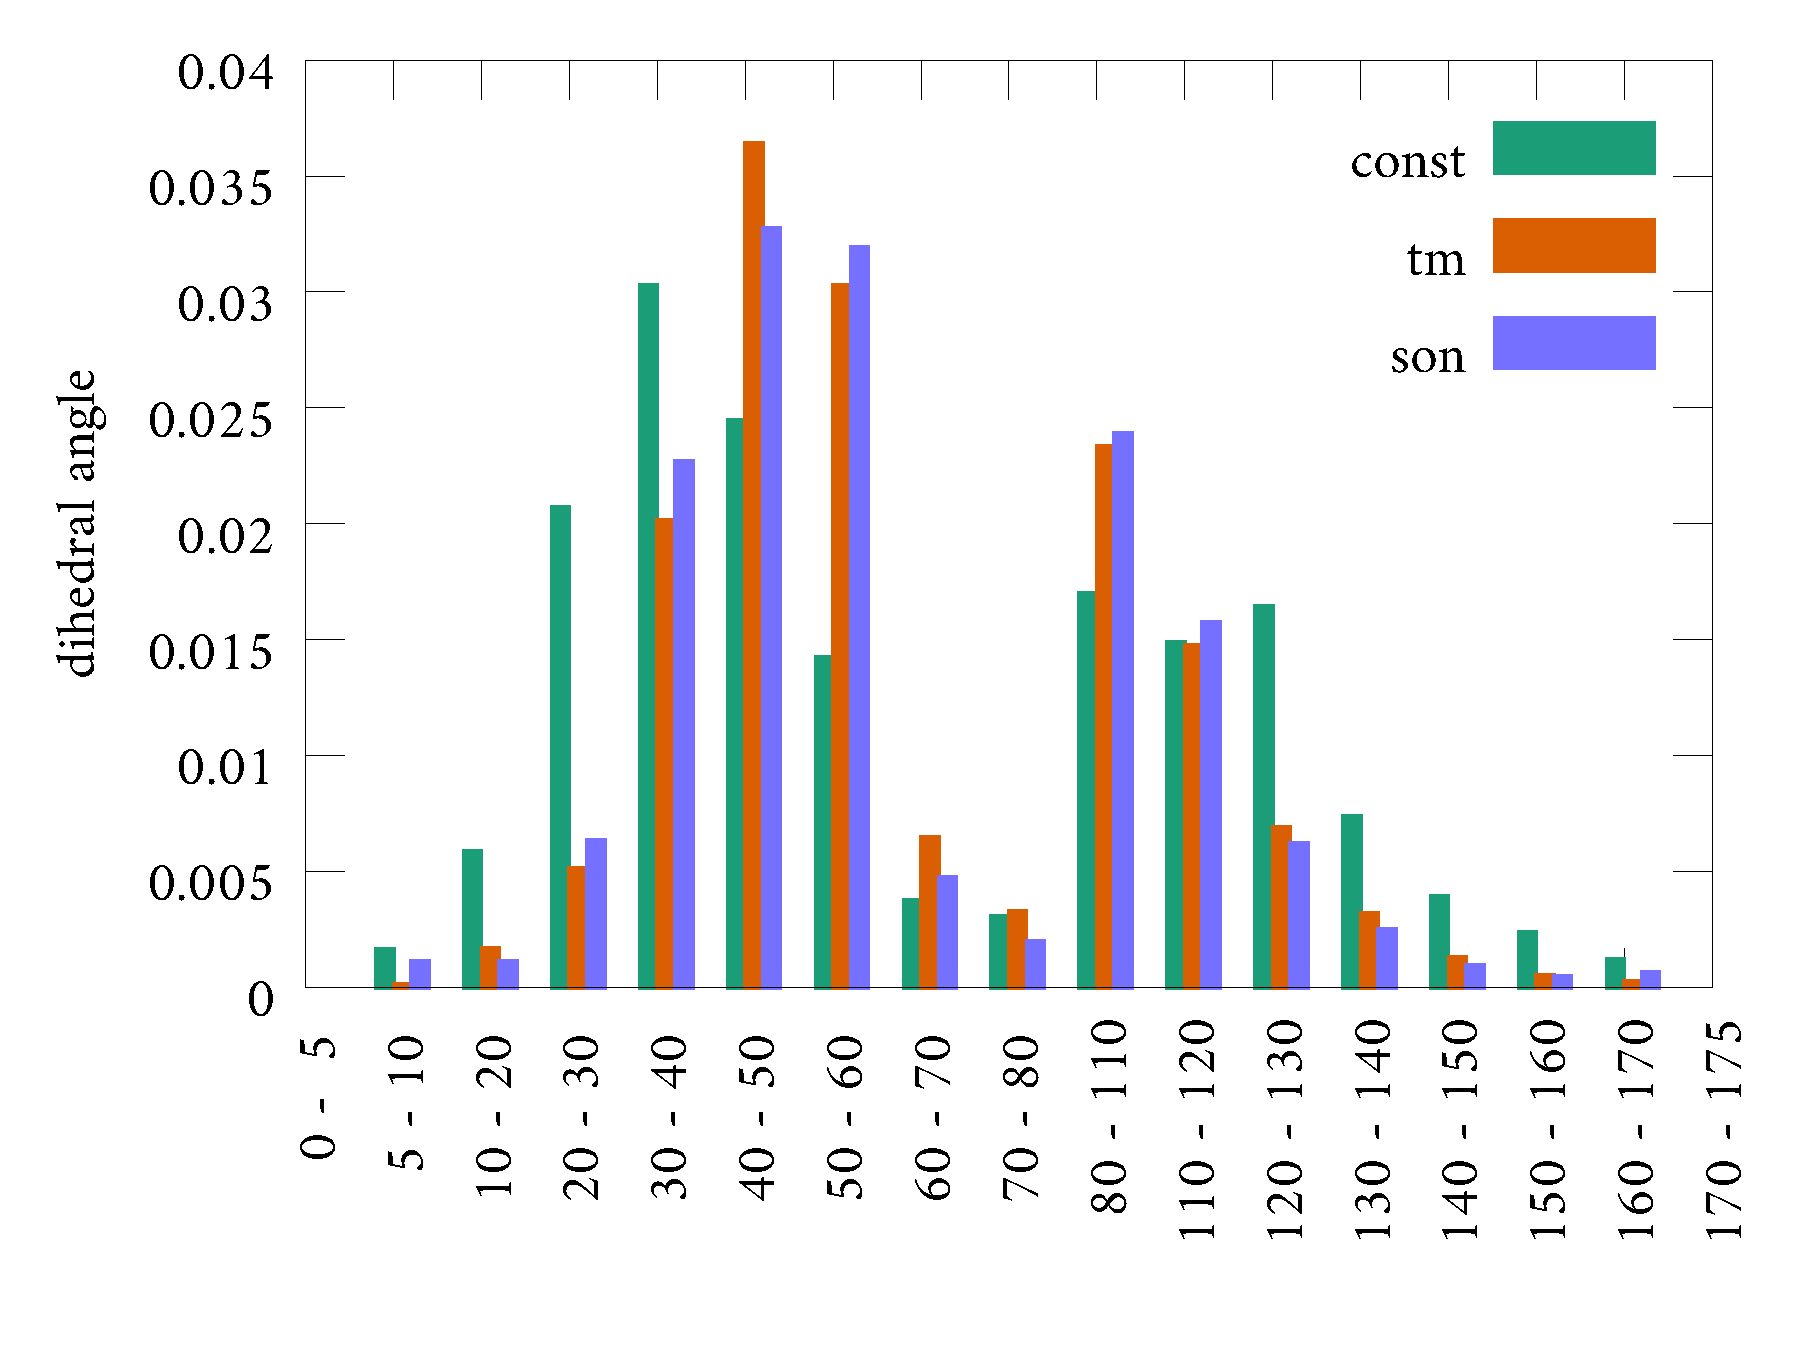
\includegraphics[width=\textwidth]{Figures/App/Rad_histAp2.pdf}
\end{subfigure}
\begin{subfigure}{0.5\textwidth}
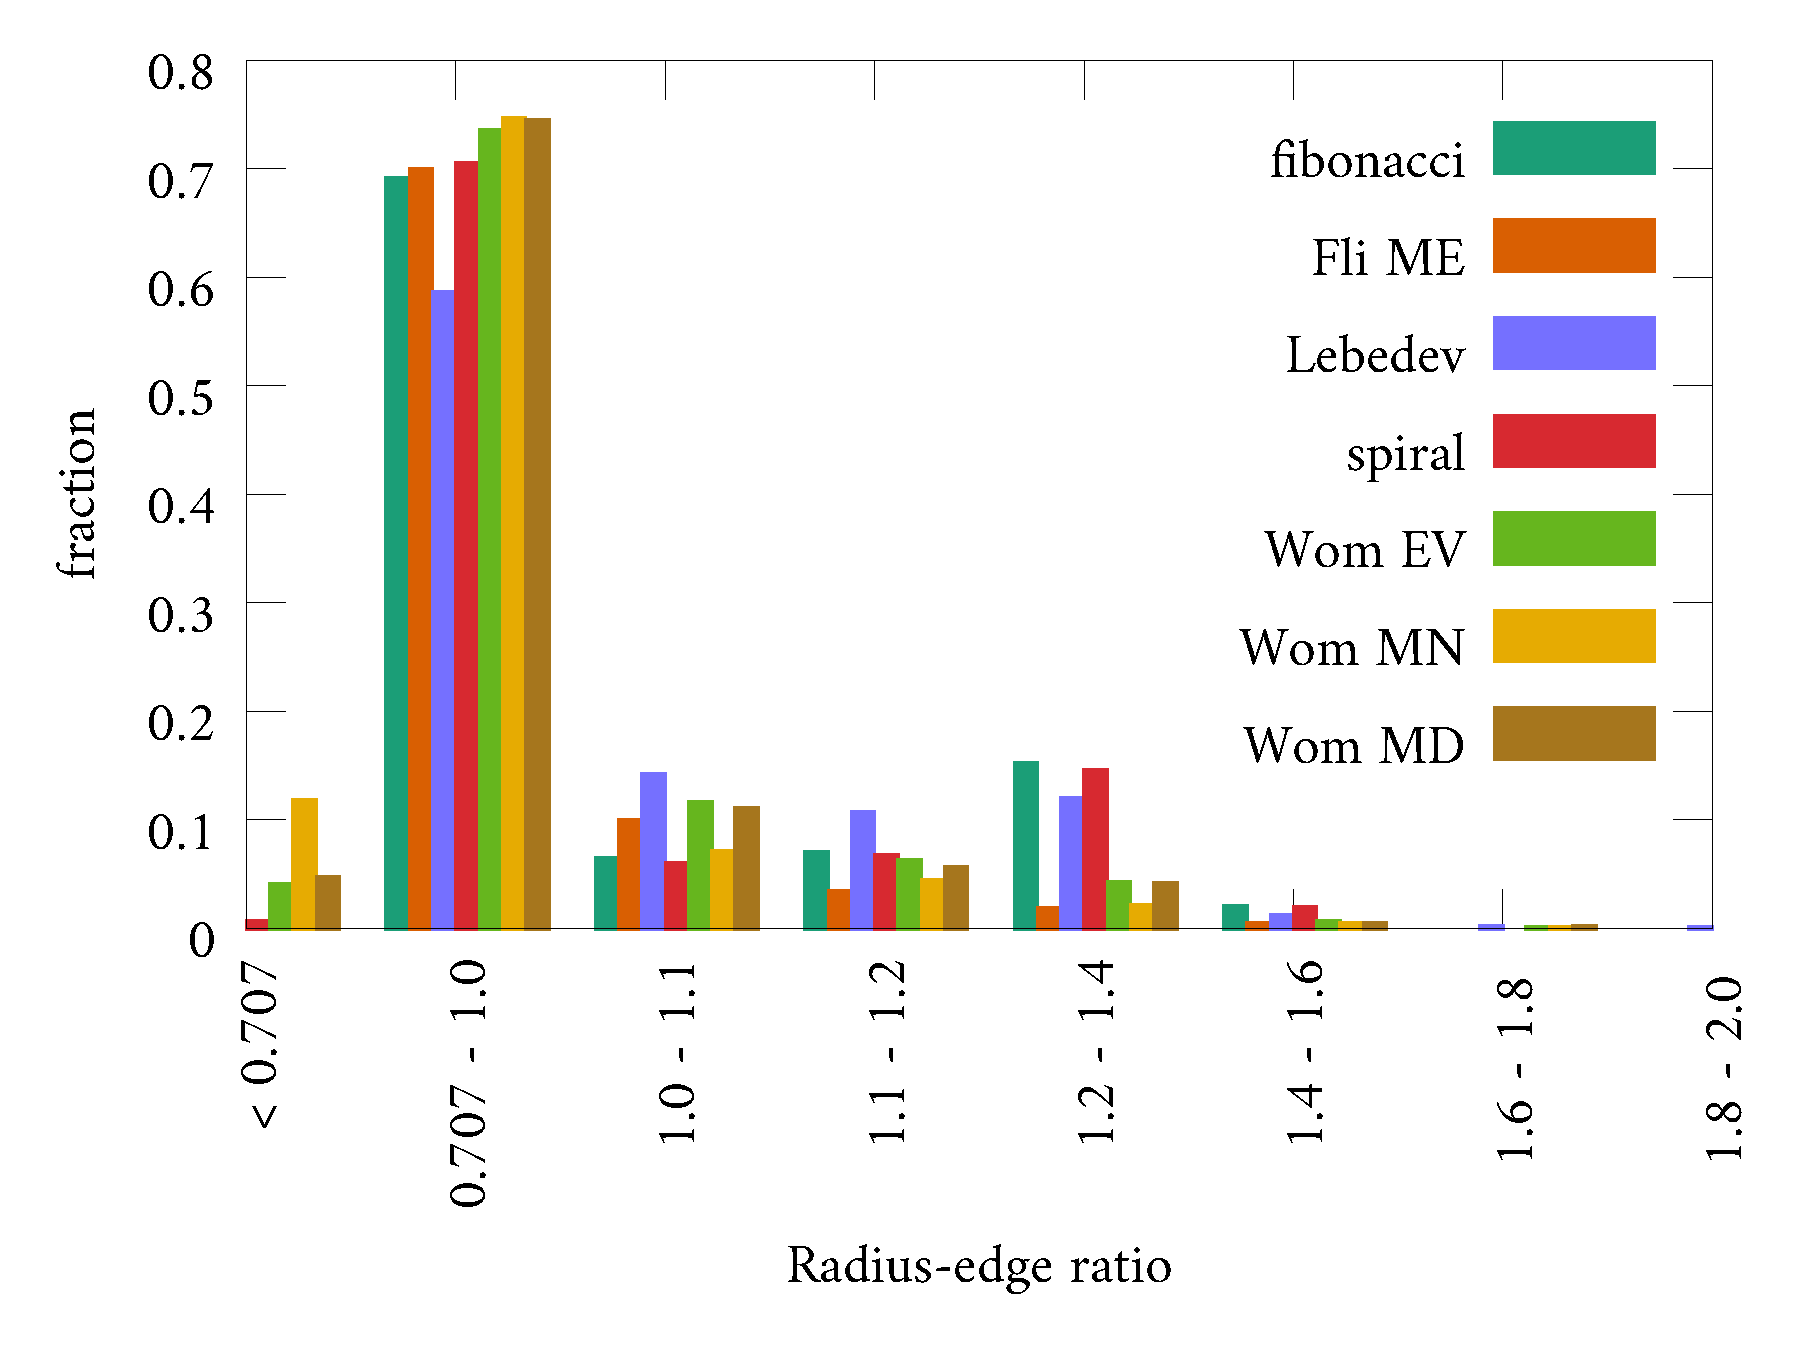
\includegraphics[width=\textwidth]{Figures/App/Sph_histAp1.pdf}
\end{subfigure}
\begin{subfigure}{0.5\textwidth}
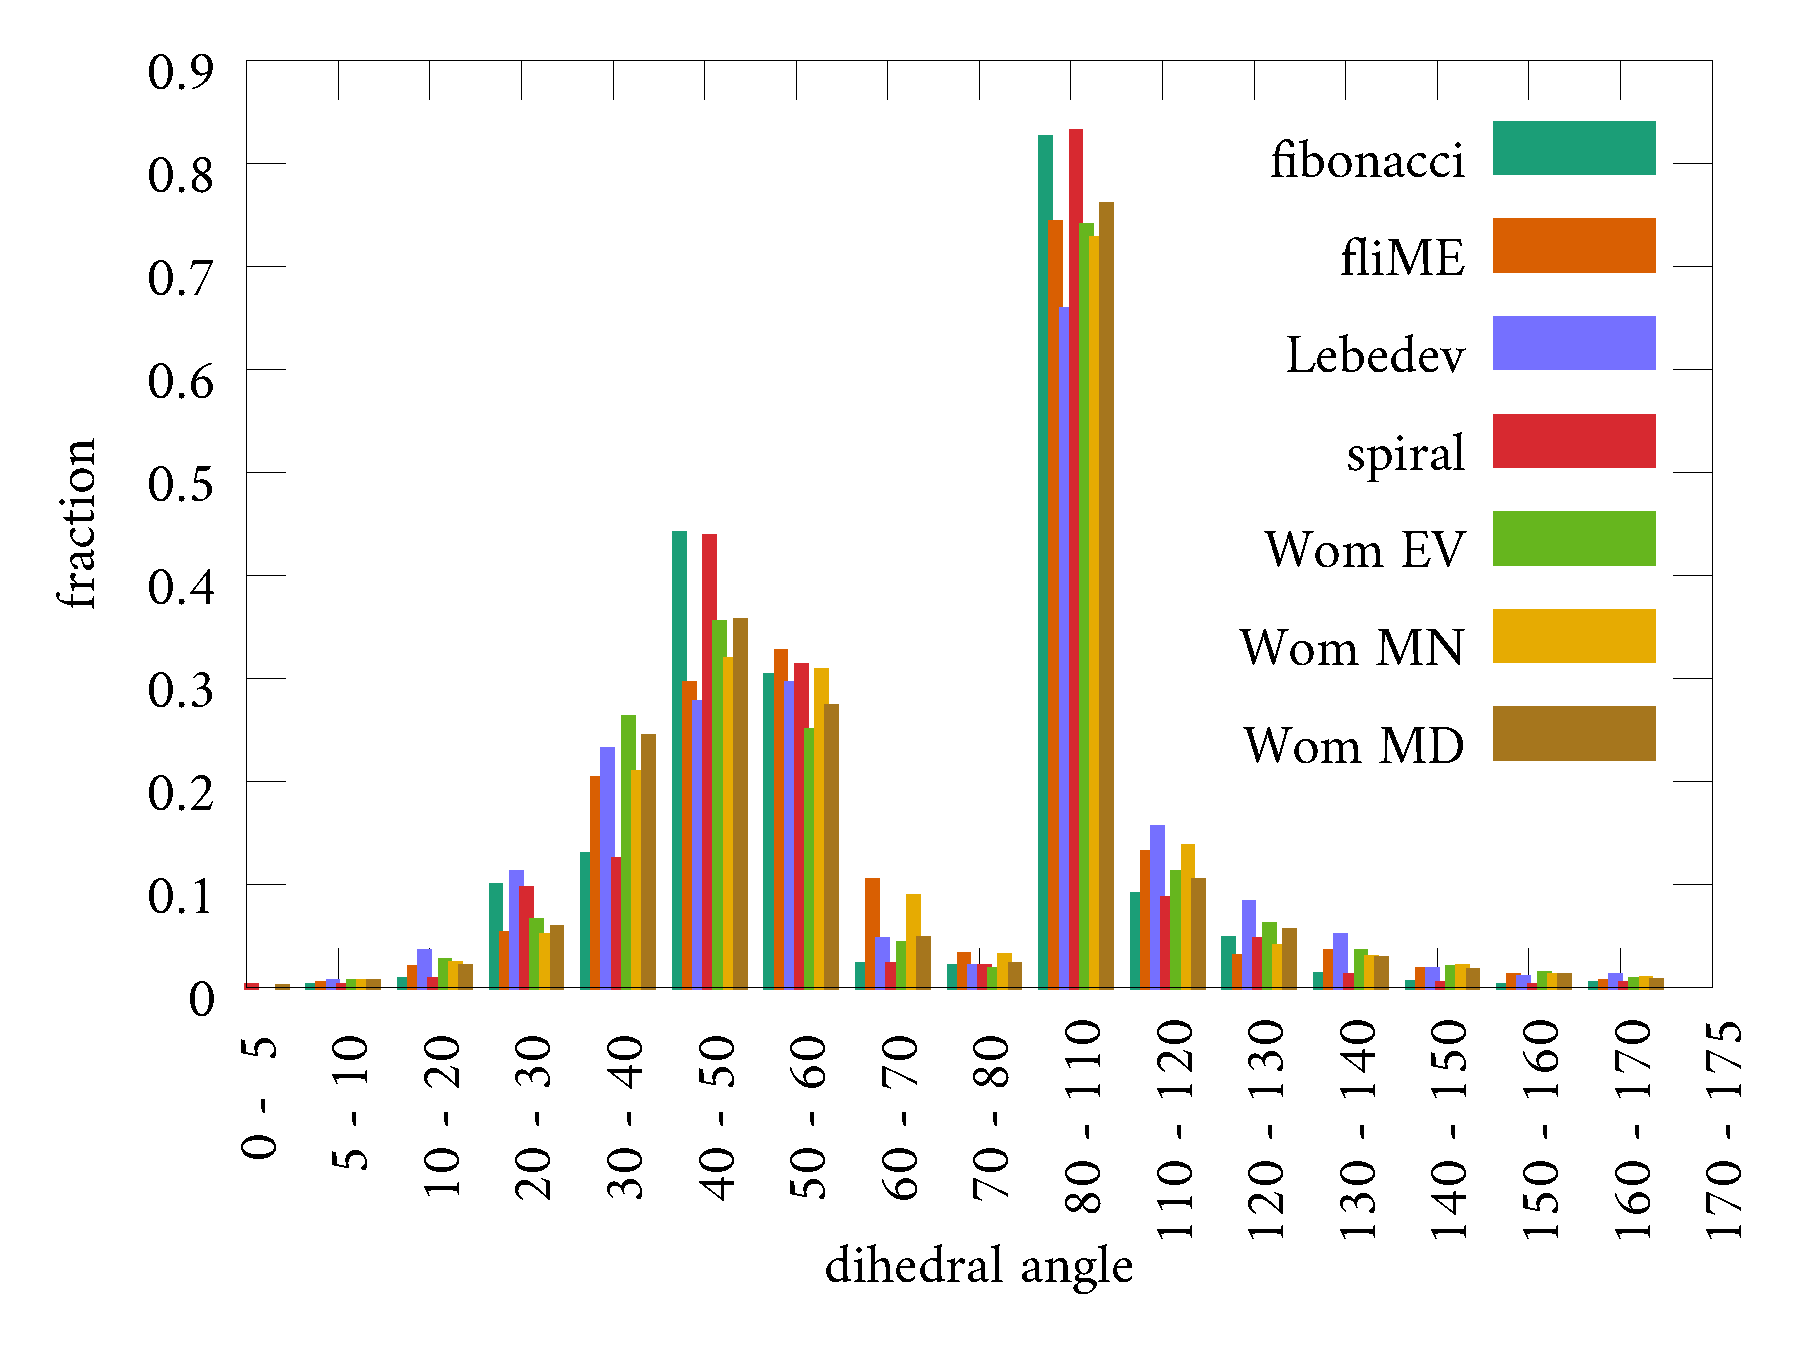
\includegraphics[width=\textwidth]{Figures/App/Sph_histAp2.pdf}
\end{subfigure}
\caption{Distribution of the ratio of radius and edge (left) and the dihedral angles (right)
for the different radial schemes (top) and angular distributions (bottom) described in section \ref{sec:NumConve}.}
\label{appFig:SchemHist}
\end{figure}

\begin{wrapfigure}{r}{0.7\textwidth}
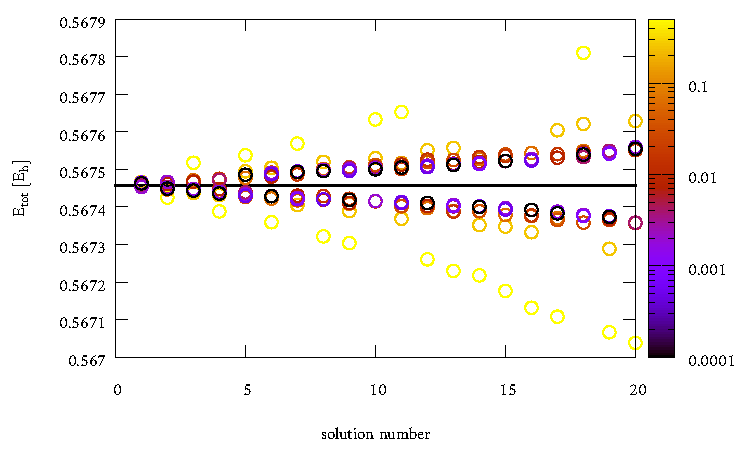
\includegraphics[width=0.7\textwidth]{Figures/IFem_powers_spectra}
\caption{The eigen energies of the first 20 solutions (circles) for different powers $p$ of the damping function $D(r)$ which determines the colours.
The spectra do not change significantly for $p<\frac 18$.}
\label{fig:powerSpect}
\end{wrapfigure}
